\documentclass[handout,nooutcomes]{ximera}
%handout
%wordchoicegiven
%space
%nooutcomes
\title{Math 160 Lab 2}
\author{Ben Sencindiver} %Used Bart Snapp and Jim Fowler's mooculus textbook as a guide
\input{preamble.tex}

\outcome{Define linear approximation as an application of the tangent to a curve.}
\outcome{Find the linear approximation to a function at a point and use it to approximate the function value.}
\outcome{Identify when a linear approximation can be used.}
\outcome{Label a graph with the appropriate quantities used in linear approximation.}
\outcome{Find the error of a linear approximation.}

\begin{document}

\section{Math 160 Lab 2 \\ Linear Approximation}

%% Have to edit the date here each semester.
\begin{abstract}
This is Lab 2 for Math 160 - Due Wednesday, March 8, 2017 at 5:00PM MST.
This lab will cover ``linear approximations'': what are they,
how do you compute them, and how are they useful. \\

Unless stated otherwise, compute all values to \underline{$6$ decimal places} in this lab.
\end{abstract}



\maketitle



%% Start with multiple choice picture question about what SHOULD a linear approximation look like?
The goal of this section of the lab is to explore and understand linear
approximations and what they {\it should} be. Linear approximations will
be important for topics in later courses such as `Newton's Method' (Calculus II),
and are the reason why in physics, sometimes you say $\sin(x)\approx x$.

\textbf{Disclaimer on this lab}:

In this lab you will be approximating function values using a technique
called linear approximation.  Most of the examples discussed in this
lab use familiar functions.  Although we may be able to evaluate the function
directly and there is no need to approximate, we will use these examples
to learn how to find linear approximations.\\


In biology systems, the function you are trying to evaluate is often
not known; you only know the way the system changes (i.e. the derivative
of the desired function) and one initial condition (i.e. the output of the
desired function at one x-value). If you want to find the function at a different
value than the one given, you may need to approximate the function value.\\

The main idea of solving such a problem is to create a linear approximation
of the function at a point you know.  From there, you can use the linear
approximation to estimate function values for points nearby. Linear
approximation is a vital tool, so we will build our intuition for
linear approximations on familiar functions. \\

\hrule
\bigskip

Now \dots to the material.\\
\medskip

Suppose you want to approximate the function $f(x) = (x-2)^2  + 4$ at $x=3$.

Let's explore what properties we would want from this approximation.\\


\textbf{Objective 1}: Play with the $m$ (slope) and $b$ (y-intercept) sliders to find
a 'good' linear approximation of $f(x)$ at $x=3$. This is not a question
that can be correct or incorrect; it is meant to build your intuition
on linear approximations.\\

\textbf{Hint}: In the desmos window below, go to an empty box in the 
desmos grapher and type `$(3,f(3))$'. This will make a `dot' at the point
on $f(x)$ that we want to approximate at. You may also want center
the point $(3, f(3))$ and zoom in to get an even better approximation.
\[
\graph[panel]{f(x) = (x-2)^2 + 4, m=0, b=0, A=mx+b}
\]

\begin{question}
Given the function $f(x)$ (in black), whose graph is below, 
what is the error of each of these various approximations
(Lines {\color{orange}A}, {\color{red}B}, {\color{blue}C }, and {\color{green}D} ) of $f(x)$ at $x=3$?

%%%% Graph%%%%%
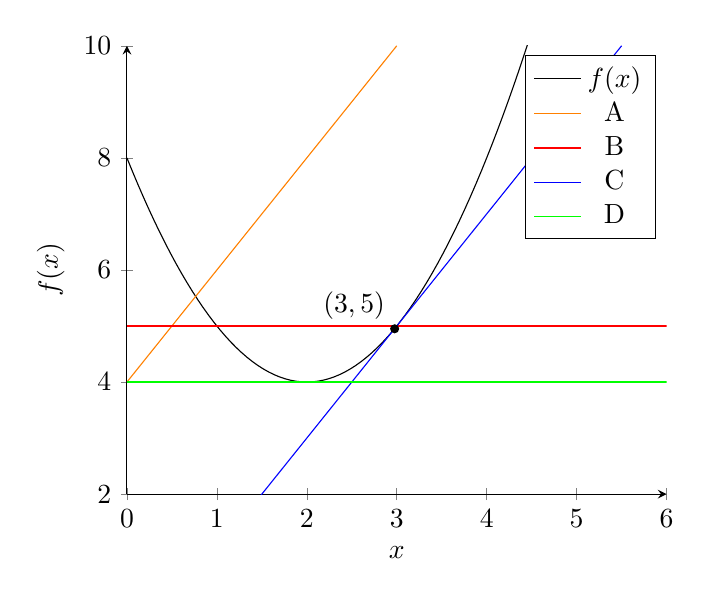
\begin{tikzpicture}
\begin{axis}[
    axis lines = left,
    xlabel = $x$,
    ylabel = {$f(x)$},
    xmin=0, xmax=6,
    ymin=2, ymax=10,
    ]
%Below the black parabola is defined
\addplot [
    domain=0:6, 
    samples=100, 
    color=black,
]
{x^2 - 4*x +8};
\addlegendentry{$f(x)$}
%Below the A approximation is defined
\addplot [
    domain=0:3, 
    samples=100, 
    color=orange,
]
{2*x +4};
\addlegendentry{A}
%Below the B approximation is defined
\addplot [
    domain=0:6, 
    samples=100, 
    color=red,
]
{0*x +5};
\addlegendentry{B}
%Below the C approximation is defined
\addplot [
    domain=-1.5:5.5, 
    samples=100, 
    color=blue,
]
{2*x -1};
\addlegendentry{C}
%Below the D approximation is defined
\addplot [
    domain=0:6, 
    samples=100, 
    color=green,
]
{0*x +4};
\addlegendentry{D}
\end{axis}
% points
\foreach \Point/\PointLabel in {(3.40,2.1)/{(3,5)}}
\draw[fill=black] \Point circle (0.05) node[above left] {$\PointLabel$};
\end{tikzpicture}
%%%%%% End of Graph%%%%

As approximations of the curve $f(x)$ at $x=3$,\\
\begin{itemize}
\item the error of Line A (given by $y=2x+4$, in orange) is $\answer{5}$\\
\item the error of Line B (given by $y=5$, in red) is $\answer{0}$\\
\item the error of Line C (given by $y=2x-1$, in blue) is $\answer{0}$\\
\item the error of Line D (given by $y=4$, in green) is $\answer{1}$\\
\end{itemize}

\begin{hint}
The `error of an approximation' is the distance between the true solution
and the approximation. (More Hints Available)
\end{hint}
\begin{hint}
If you are approximating $f(x)$ at $x=3$, then the `true solution' is the
true value of $f(x)$ at $x=3$, AKA $f(3)$. (More Hints Available)
\end{hint}
\begin{hint}
The approximation of the function $f(x)$ at $x=a$ using a line 
$y=mx+b$ is $ma+b$.(More Hints Available)
\end{hint}
\begin{hint}
Error shouldn't be negative. If you are finding the difference
between two numbers and the difference is negative, then the absolute
value of the difference would give the distance between the numbers.
\end{hint}
\end{question}

\begin{question}
Given the errors you found for $f(x)$ at $x=3$ using  each line (A,B,C, and D), which line(s) has (have) the least error at $x=3$?
\begin{selectAll}
\choice{A}
\choice[correct]{B}
\choice[correct]{C}
\choice{D}
\end{selectAll}
\end{question}

%% Justifying that Linear Approximations go through the point you are approximating at.

This establishes an important property of a linear approximation
of a function at a given point: {\it the best linear approximation
should agree with the point at which you are approximating.}
In other words, if you are approximating a function $f(x)$ at $x=a$ with a
line $\l(x)$, then the line should be such that $\l(a)=f(a)$;
the output of the line is the same as the function's output at the $x$-value you are approximating at.\\

%%% Justifying the slope of the approximation
\textbf{Question}: What is the difference between two lines that both
have no error where you are approximating at?
Consider the graph of $f(x)= (x-2)^2 + 4$ (in black), and three other linear approximations.

%%%%%% Graph 2 %%%%%
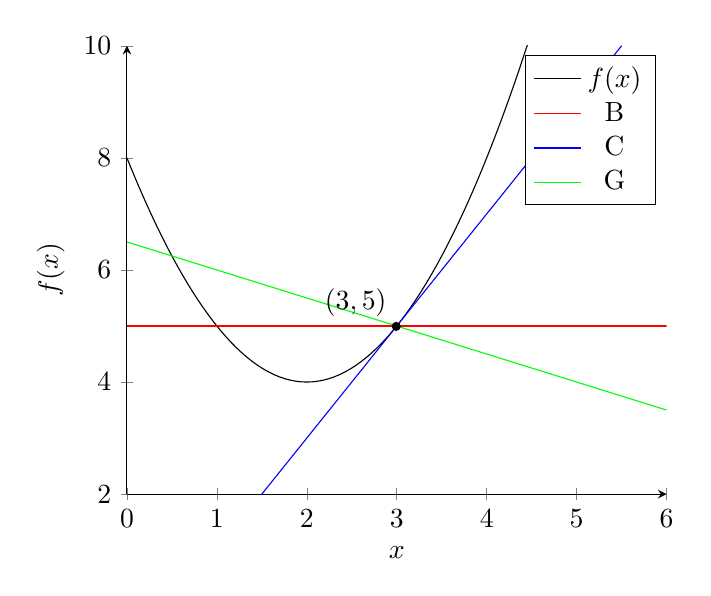
\begin{tikzpicture}
\begin{axis}[
    axis lines = left,
    xlabel = $x$,
    ylabel = {$f(x)$},
    xmin=0, xmax=6,
    ymin=2, ymax=10,
    ]
%Below the black parabola is defined
\addplot [
    domain=0:6, 
    samples=100, 
    color=black,
]
{x^2 - 4*x +8};
\addlegendentry{$f(x)$}
%Below the B approximation is defined
\addplot [
    domain=0:6, 
    samples=100, 
    color=red,
]
{0*x +5};
\addlegendentry{B}
%Below the C approximation is defined
\addplot [
    domain=-1.5:5.5, 
    samples=100, 
    color=blue,
]
{2*x -1};
\addlegendentry{C}
%Below the G approximation is defined
\addplot [
    domain=0:6, 
    samples=100, 
    color=green,
]
{-0.5*x +6.5};
\addlegendentry{G}
\end{axis}
% points
\foreach \Point/\PointLabel in {(3.42,2.13)/{(3,5)}}
\draw[fill=black] \Point circle (0.05) node[above left] {$\PointLabel$};
\end{tikzpicture}
%%%%%% End of Graph 2 %%%%%%

\begin{question}
Let's ask another question: What are the errors of the approximations `near' $x=3$? \\

%%% Approx at x=2.9
Given the new graph above, then as approximations of the curve $f(x)$ at {\bf $x=2.9$},
\begin{itemize}
\item the error of Line B (given by $y=5$, in red) is $\answer{0.19}$
\item the error of Line C (given by $y=2x-1$, in blue) is $\answer{0.01}$
\item the error of Line G (given by $y=-0.5*x + 6.5$, in green) is $\answer{0.24}$
\end{itemize}

\textbf{Hint}: Though you can do the computations by hand, use the
desmos calculator below to help with the computations. 
Note that that $f(2.9)$ is given for you. Alter this to get what you're looking for!\\
Click the `Reveal Hint' button to learn how to evaluate the functions using
the desmos calculator.\\
\begin{hint}
Typing `$B(3)$' into a blank entry on the desmos calculator
evaluates the line $B$ at $x=3$. (More Hints Available)
\end{hint}
\begin{hint}
Typing `$|f(4.1) - G(4.1)|$' would compute the error of the approximation
of $f(x)$ at $x=4.1$ using the line $G$.
\end{hint}
\[
\graph[panel]{C(x) = 2x -1, G(x) = -0.5x + 6.5, f(x) = (x - 2)^2 + 4, B(x) = 0x + 5,  f(2.9)}
\]

\medskip
%%%%% Approx at x=3.1

Use the desmos calculator above to answer the following questions.

As approximations of the curve $f(x)$ at {\bf $x=3.1$},\\
\begin{itemize}
\item the error of Line B (given by $y=5$, in red) is $\answer{0.21}$\\
\item the error of Line C (given by $y=2x-1$, in blue) is $\answer{0.01}$\\
\item the error of Line G (given by $y=-0.5*x + 6.5$, in green) is $\answer{0.26}$\\
\end{itemize}
\end{question}

\begin{question}
Given the errors you found for $f(x)$ at $x=2.9$ and $x=3.1$ using the lines B,C, and G, which line(s) has (have) the least error `near' $x=3$?
\begin{selectAll}
\choice{B}
\choice[correct]{C}
\choice{G}
\end{selectAll}
\end{question}

\textbf{Warning}: `Near' is not a well-defined notion. $2.99$ is closer than $2.9$
to $3$, and
$2.999$ is even closer to $3$ than $2.99$. We are merely trying to get 
an idea for what is happening graphically: if we mentally `zoom' in 
near the point $(3,5)$, we want our linear approximation to
be as close as possible to the function we are approximating, in this case $f(x) = (x-2)^2 + 4$.\\
\hrule
\medskip

Now what's so special about the linear approximation above? 
What is the slope of that line? It looks like the slope of best linear
approximation of the $f(x)$ at $x=3$ is $f'(3)$. This is no coincidence! 
The best linear approximation of a differential function at $x=a$
is precisely the tangent line to the curve at $x=a$! We have just found our last important property of our \textit{best} linear approximation at $x=a$: The slope of the best linear approximation of a function $f(x)$ at $x=a$ is the slope of the line tangent to $f(x)$ at $x=a$, i.e. the derivative of evaluated at $x=a$ ($f'(a)$)!\\
\medskip


Given a function, a \textit{linear approximation} (at $x=a$) is a fancy phrase
for something you already know:
\begin{center}
\begin{quote}
  \textbf{The line tangent to the function (at $x=a$).}
\end{quote}
\end{center}


\begin{definition}
If $f$ is a differentiable function at $x=a$, then a \textbf{linear
  approximation} for $f$ at $x=a$ is given by
\[
\l(x) = f'(a)(x-a) +f(a).\\
\]
\end{definition}


%%%%% Should there be an example here?




Note that $\l(x)$ is just the line tangent to $f(x)$ at $x=a$.


\begin{example}
Below is the graph of $f(x) = 1/8x^3 + (3/8)x^2 -3/4 - 2$ and the line
tangent to $f(x)$ at $x=a$. Feel free to explore how the tangent line
(in purple) changes as $a$ varies by using the slider. You may need to
hit `-' (zoom out) in order to see the linear approximations for large $a$ values.
\[
\graph[panel]{a=1, f(x) = 1/8x^3 + (3/8)x^2 -3/4 - 2, t(x) = f'(a)(x-a)+ f(a)}
\]

Notice how the linear approximation (the purple line) tangentially hugs
$f(x)$ (the green line) at the $x=a$ value!
\end{example}


\end{document}
